% !TeX spellcheck = en_GB
\documentclass[11pt]{article}

% Use the header
% Use ngerman instead of british if you want to write yor report in german
\usepackage[british]{babel}
\usepackage[utf8]{inputenc}
\usepackage{geometry}
% math stuff
\usepackage{amsmath}
\usepackage{amssymb}
% Customization of ordered and unordered lists
\usepackage{enumitem}
% Include nicely formatted code in your latex documents
\usepackage{listings}
\usepackage{color}
% Nice looking tables
\usepackage{booktabs}
% Add glaring red TODO notes to your docuemnt
\usepackage{todonotes}
% Use biber instead of the antique bibtex
% You might need to change some settings in your editor for that to work correctly
% In Texstudio go to 'Options'->'Configure Texstudio...'->'Build' and set 'Default Bibliography Tool' to 'Biber'
\usepackage[backend=biber,style=numeric-comp,sorting=none]{biblatex}
% Extended customization of floats, like figures, tables, etc.
\usepackage{float}
% Better support for including figures
\usepackage{graphicx}
% Hyperlinking within the document and support for external links
\usepackage{hyperref}
% Automatically infer the type of reference
\usepackage{cleveref}
% Including url and hyperlinks in the document
\usepackage{hyperref}

\geometry{a4paper}

% Uncomment this to allow multiline equation to extend to multiple pages
%\allowdisplaybreaks

% Remove extra space between figures and captions.
\setlength{\abovecaptionskip}{0pt}

% Unicode workaround for lstlistings
\lstset{literate=
	{á}{{\'a}}1 {é}{{\'e}}1 {í}{{\'i}}1 {ó}{{\'o}}1 {ú}{{\'u}}1
	{Á}{{\'A}}1 {É}{{\'E}}1 {Í}{{\'I}}1 {Ó}{{\'O}}1 {Ú}{{\'U}}1
	{à}{{\`a}}1 {è}{{\`e}}1 {ì}{{\`i}}1 {ò}{{\`o}}1 {ù}{{\`u}}1
	{À}{{\`A}}1 {È}{{\'E}}1 {Ì}{{\`I}}1 {Ò}{{\`O}}1 {Ù}{{\`U}}1
	{ä}{{\"a}}1 {ë}{{\"e}}1 {ï}{{\"i}}1 {ö}{{\"o}}1 {ü}{{\"u}}1
	{Ä}{{\"A}}1 {Ë}{{\"E}}1 {Ï}{{\"I}}1 {Ö}{{\"O}}1 {Ü}{{\"U}}1
	{â}{{\^a}}1 {ê}{{\^e}}1 {î}{{\^i}}1 {ô}{{\^o}}1 {û}{{\^u}}1
	{Â}{{\^A}}1 {Ê}{{\^E}}1 {Î}{{\^I}}1 {Ô}{{\^O}}1 {Û}{{\^U}}1
	{œ}{{\oe}}1 {Œ}{{\OE}}1 {æ}{{\ae}}1 {Æ}{{\AE}}1 {ß}{{\ss}}1
	{ű}{{\H{u}}}1 {Ű}{{\H{U}}}1 {ő}{{\H{o}}}1 {Ő}{{\H{O}}}1
	{ç}{{\c c}}1 {Ç}{{\c C}}1 {ø}{{\o}}1 {å}{{\r a}}1 {Å}{{\r A}}1
	{€}{{\euro}}1 {£}{{\pounds}}1 {«}{{\guillemotleft}}1
	{»}{{\guillemotright}}1 {ñ}{{\~n}}1 {Ñ}{{\~N}}1 {¿}{{?`}}1
}

% Define Synatx highlighting for Python
\definecolor{maroon}{cmyk}{0, 0.87, 0.68, 0.32}
\definecolor{halfgray}{gray}{0.55}
\definecolor{ipython_frame}{RGB}{207, 207, 207}
\definecolor{ipython_bg}{RGB}{247, 247, 247}
\definecolor{ipython_red}{RGB}{186, 33, 33}
\definecolor{ipython_green}{RGB}{0, 128, 0}
\definecolor{ipython_cyan}{RGB}{64, 128, 128}
\definecolor{ipython_purple}{RGB}{170, 34, 255}

\lstdefinelanguage{iPython}{
	morekeywords=[1]{access,and,break,class,continue,def,del,elif,else,except,exec,finally,for,from,global,if,import,in,is,lambda,not,or,pass,print,raise,return,try,while},%
	%
	% Built-ins
	morekeywords=[2]{abs,all,any,basestring,bin,bool,bytearray,callable,chr,classmethod,cmp,compile,complex,delattr,dict,dir,divmod,enumerate,eval,execfile,file,filter,float,format,frozenset,getattr,globals,hasattr,hash,help,hex,id,input,int,isinstance,issubclass,iter,len,list,locals,long,map,max,memoryview,min,next,object,oct,open,ord,pow,property,range,raw_input,reduce,reload,repr,reversed,round,set,setattr,slice,sorted,staticmethod,str,sum,super,tuple,type,unichr,unicode,vars,xrange,zip,apply,buffer,coerce,intern},%
	%
	sensitive=true,%
	morecomment=[l]\#,%
	morestring=[b]',%
	morestring=[b]",%
	%
	morestring=[s]{'''}{'''},% used for documentation text (mulitiline strings)
	morestring=[s]{"""}{"""},% added by Philipp Matthias Hahn
	%
	morestring=[s]{r'}{'},% `raw' strings
	morestring=[s]{r"}{"},%
	morestring=[s]{r'''}{'''},%
	morestring=[s]{r"""}{"""},%
	morestring=[s]{u'}{'},% unicode strings
	morestring=[s]{u"}{"},%
	morestring=[s]{u'''}{'''},%
	morestring=[s]{u"""}{"""},%
    morestring=[s]{f'}{'},% format strings
    morestring=[s]{f"}{"},%
    morestring=[s]{f'''}{'''},%
    morestring=[s]{f"""}{"""},%
	%
	identifierstyle=\color{black}\ttfamily,
	commentstyle=\color{ipython_cyan}\ttfamily,
	stringstyle=\color{ipython_red}\ttfamily,
	keepspaces=true,
	showspaces=false,
	showstringspaces=false,
	%
	rulecolor=\color{ipython_frame},
	frame=single,
	frameround={t}{t}{t}{t},
	framexleftmargin=6mm,
	numbers=left,
	numberstyle=\tiny\color{halfgray},
	%
	%
	backgroundcolor=\color{ipython_bg},
	extendedchars=true,
	basicstyle={\small\ttfamily},
    keywordstyle=[1]{\color{ipython_green}\ttfamily},
	keywordstyle=[2]{\color{ipython_purple}\ttfamily},
}

% General math commands
\newcommand{\argmin}{\operatornamewithlimits{arg\ min}}
\newcommand{\argmax}{\operatornamewithlimits{arg\ max}}
\newcommand{\img}{\operatorname{Im}}
\newcommand{\dotcup}{\mathbin{\dot{\cup}}}

% Probability commands
\newcommand{\expect}[2][{}]{\operatornamewithlimits{\mathbb{E}}_{#1}\left[#2\right]}
\newcommand{\prob}[2][{}]{\operatornamewithlimits{\mathbb{P}}_{#1}\left[#2\right]}
\newcommand{\Var}{\operatorname{Var}}
\newcommand{\Cov}{\operatorname{Cov}}
\newcommand{\Ind}[1]{\operatorname{\mathbb{I}}_{#1}}

% Calculus commands
\newcommand{\norm}[1]{\left\lVert#1\right\rVert}

% Add this at the end of a line of an unnumbered multiline equation
% It will produce a single equation nuber just for that line
\newcommand\numberthis{\addtocounter{equation}{1}\tag{\theequation}}


% Add bib file that contains references
\addbibresource{references.bib}

\title{Machine Learning Project\\Task 1 Report Template}
\author{Philipp Liznerski \\ liznerski@cs.uni-kl.de\and
	Tobias Michels\\ t\_michels15@cs.uni-kl.de\and
    Saurabh Varshneya\\ varshneya@cs.uni-kl.de}
\date{\today}
\begin{document}
	
\maketitle

\section{HOW-TO}
This template aims at less experienced \LaTeX users and shows how to achieve some common tasks that might come up as you are writing your report. We don't require you to use the template; if you want, you can simply delete it and start your report from scratch or use your own template files.

\subsection{Equations}
We can easily typeset equations over multiple lines using the \verb|align| environment, however this will add a number to the end of every single line. The \verb|align*| environment on the other hand does not add numbers to any of the equations, but we can use the \verb|\numberthis| command at the end of a line to give only that line a number:
\begin{align*}
	2 + 2 &= 4\\
	4 - 1 &= 3 \numberthis \label{eq:quickmaths}
\end{align*}
Now we can reference the second line as \cref{eq:quickmaths} using the \verb|\cref| command. Note that the \texttt{cleveref} package automatically determined that the type of object we wanted to reference is an equation and it therefore added the corresponding text. \Cref{eq:quickmaths} can also be referenced at the beginning of a sentence if we use the \verb|\Cref| command instead.

\subsection{Ordered Lists}
The \verb|enumitem| packages provides great flexibility in handling ordered lists, specifically \verb|enumerate| environments. Usually, items would be labelled by Arabic numbers and a period:
\begin{enumerate}
    \item This
    \item is
    \item a test.
\end{enumerate}
Perhaps you would like to have letters instead to replicate the task sheet and not quite as much empty space between the items? Not a problem:
\begin{enumerate}[itemsep=0.0em, label=\alph*)]
    \item This
    \item is
    \item a test.
\end{enumerate}
Spacing can also be adjusted globally, using the command \verb|\setlist{itemsep=<spacing>}|.

\subsection{Figures \& Code}
At some point, you might want to include plots or other graphics in your report. Usually, this is done by defining a figure that does not necessarily appear at the point in the document where it was defined; see \cref{fig:functions} for example. The python code that generated the figure is also included with the report template, please have a look at the file \verb|figures/make_figures.py|.

\begin{figure}[t]
    \begin{center}
        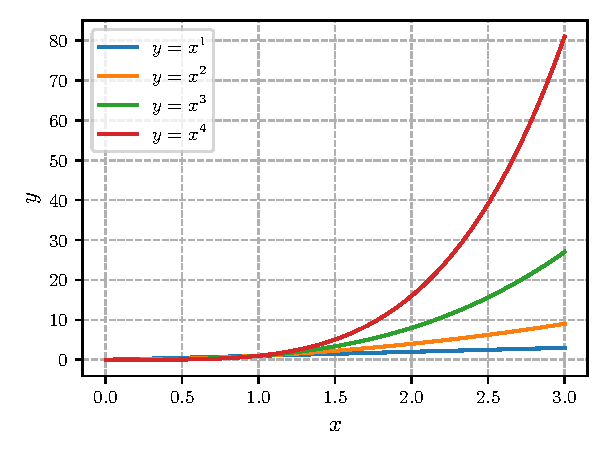
\includegraphics{figures/example_plot}
    \end{center}
    \caption{A figure that shows the relationship between $y$ and $x$.}
    \label{fig:functions}
\end{figure}

But what if you want to include and reference parts of your code in the report? In that case, you can use the \verb|lstlisting| environment, which enables you to typeset code directly in \LaTeX. The header file comes with an updated definition of the python language, which supports syntax highlighting for most parts of the language. Here is a small example:
\begin{lstlisting}[language=iPython]
def count_ones(bits: int) -> int:
    # count number of ones in the binary representation 
    # of the signed integer bits   
    c = 0
    v = bits
    while v != 0:
        c += 1
        v &= v - 1  # This clears the least significant 1 bit
        
    return c
\end{lstlisting}

Instead of writing the code directly in the \LaTeX file, you can also ``import'' it from the original source file with the \verb|\lstinputlisting| command. For example, \cref{lst:figsource} shows an excerpt from the source code file \verb|figures/make_figures.py| that was used to generate \cref{fig:functions}.

Note how the code about counting bits was split up between two separate pages. This is expected behaviour, since the normal text mode works like a paragraph of text, which can obviously be split. If you don't want that behaviour, use the optional \verb|float| parameter that turns the listing into a floating object, similar to a figure. For example, \cref{lst:figsource} uses this parameter and is not split between two pages, but at the same time the source code does not appear in the exact position where it was included in the \LaTeX file.

\lstinputlisting[float=tb, language=iPython, firstline=43, lastline=59, caption={Source code that generated \cref{fig:functions}.}, label=lst:figsource]{figures/make_figures.py}

\subsection{TODO Notes}
\todo[inline]{TODO: Remove this TODO note}
Notes and reminders like the one above can by typeset with the \verb|\todo[inline]{<text>}| command\todo{Mention that notes can also be added next to the text area}. This is especially helpful if you are collaborating with others, since you can use this to remind everyone of work that still needs to be done.

\subsection{Citing References}
If you want to use material created by someone else in your report, it is mandatory that you cite it properly. This is even more important if you want to refer to somebody else's ideas. Luckily, \LaTeX and the internet can help you with that, making your life a lot easier in that regard. Ideally, you would only want to cite papers that were published either in a peer-reviewed journal or a conference's proceedings. For example, you might have read the OpenAI blog post about \emph{adversarial examples}\footnote{\url{https://openai.com/blog/adversarial-example-research/}} and you want to pick up some of the ideas presented there. Since the blog post lists the relevant papers, you can search for them in an engine like \emph{Google Scholar} that lets you export citations as \emph{BibTeX} entries. After pasting the entry in your references file, you can cite them in your text by simply using the \verb|\autocite| command: \autocite{papernot2017practical}.

Of course, finding a peer-reviewed paper for the ideas in a blog post might not always be possible. In such a case, you can also cite the blog post directly using an \verb|@online| entry in the bib file \autocite{goodfellow2017attacking}. 

% Print references
\printbibliography
\end{document}